\documentclass[ngerman,a4paper]{texmf/tex/latex/mathscript/mathscript}
\usepackage{texmf/tex/latex/mathoperators/mathoperators}

\title{\textbf{Interpolation der \person{Runge}-Funktion und anderer Funktionen mit Octave}}
\author{\person{Henry Haustein}, \person{Lars Ortscheidt}}

\begin{document}
\maketitle
	
\tableofcontents
\pagebreak
	
\section{Interpolation der \person{Runge}-Funktion}	
	\begin{align}
		f(x) = \frac{1}{1+25x^2}\notag
	\end{align}
	
	\subsection{Berechnung der Splines}
	\subsubsection{Polynomsplines aus $\mathcal{S}_1^0(\Delta)$}
	
	Eine Polynomspline $s\in\mathcal{S}_1^0(\Delta)$ ist eine affin lineare Funktion, das heißt er hat die Form $s(x)=mx+n$ mit Anstieg $m$ und $y$-Achsenverschiebung $n$. 
	
	Die Interpolationsfunktion $g_N$, mit $N+1$ Stützstellen, besteht nun also aus Splines $s_i\in\mathcal{S}_1^0(\Delta)$, wobei für jeden Spline gilt:
	\begin{align}
		\text{Definitionsbereich: } & [x_i,x_{i+1}] \notag \\
		m_i =& \frac{f_{i+1}-f_i}{x_{i+1}-x_i}\notag \\
		n_i =& f_i \notag
	\end{align} 
	wobei $x_i$ die Stützstellen und $f_i$ die Stützwerte sind. Dabei läuft $i$ von $0$ bis $N-1$.
	
	Der Quelltext für Octave sieht dann so aus:
\begin{lstlisting}
runge = @(x) 1./(1+25*x.^2);
xreal = -1:0.01:1;

n = input('Anzahhl der Stuetzstellen - 1 := N: ');

%Schritweite h berechnen
h = 2/n
%Stuetzstellenvektor x berechnen
x = -1:h:1;

for i=1:n+1
 %Stutzwertevektor f berechnen
 f(i) = runge(x(i));
endfor

for i=1:n
 %Anstiege m_i berechnen
 m(i) = (f(i+1)-f(i))./(x(i+1)-x(i));
 %Achsenabschnitte n_i berechnen
 n(i) = f(i);
endfor

plot(x, f, "-;Interpol.;", xreal, runge(xreal), "-;Rungefkt.;")
\end{lstlisting}

	Das Interessante hierbei ist, dass die berechneten Werte in den Arrays \texttt{m} und \texttt{n} gar nicht für die Interpolation gebraucht werden - die Funktion \texttt{plot} interpoliert automatisch linear, wenn man ihr die Stützstellen und -werte übergibt.
	
	\begin{figure}[h]
		\centering
		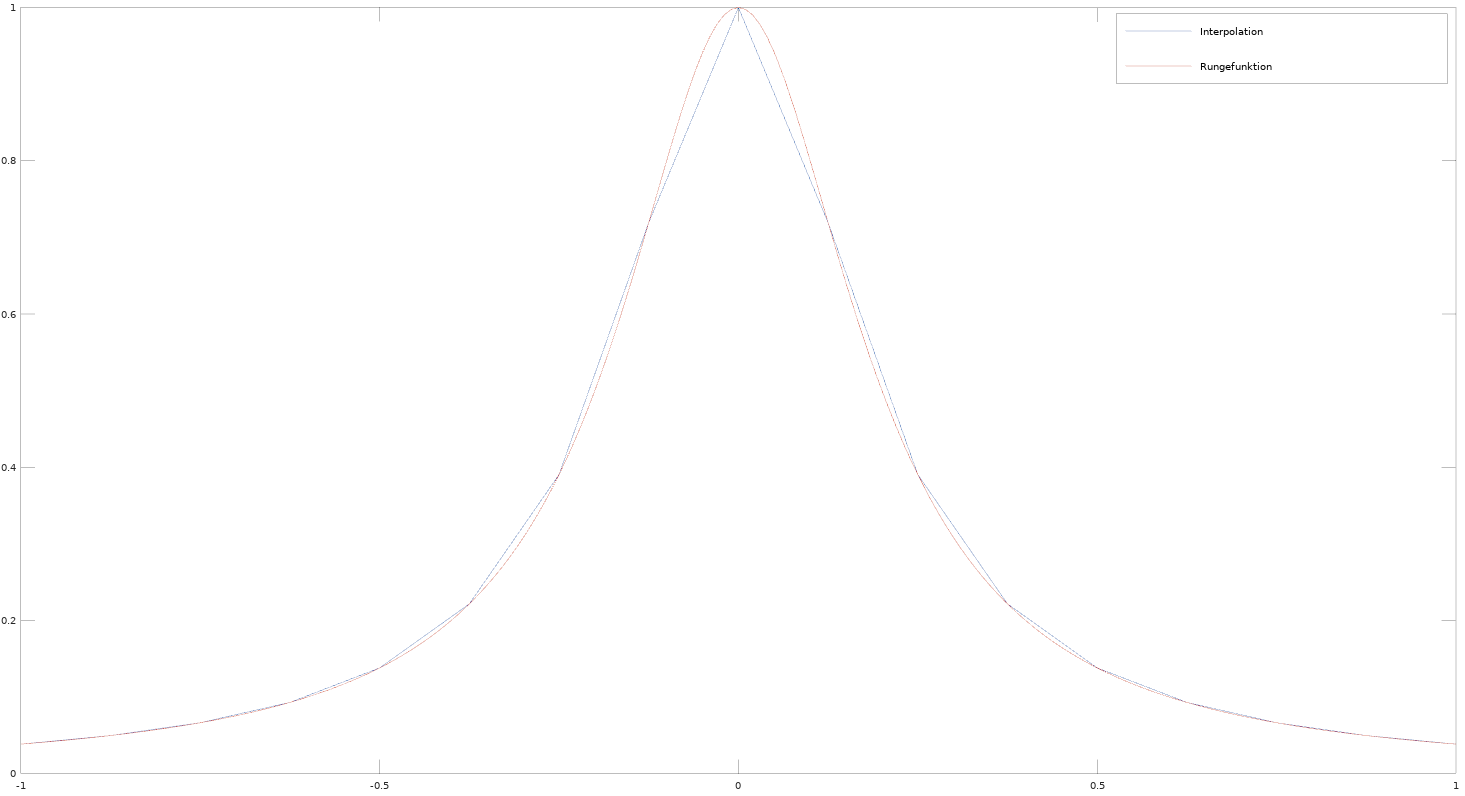
\includegraphics[width=0.9\textwidth]{images/Runge_lineare_Interpolation.png}
		\caption{lineare Splineinterpolation mit $N=16$}
	\end{figure}
	
	\subsubsection{Polynomsplines aus $\mathcal{S}_3^1(\Delta)$}
	
	\subsection{Fehlerbetrachtung}
	
	\subsection{Diskussion der Ergebnisse}


\section{Interpolation der anderen Funktion}
	\begin{align}
		f(x) &= \left( 1+\cos\left(\frac{3}{2}\pi x \right) \right)^{\sfrac{2}{3}}\notag \\
		f'(x) &=-\frac{\pi\sin\left(\frac{3}{2}\pi x\right)}{\sqrt[3]{1+\cos\left(\frac{3}{2}\pi x \right)}}\notag
	\end{align}
	
	\subsection{Berechnung der Splines}
	\subsubsection{Polynomsplines aus $\mathcal{S}_1^0(\Delta)$}
	
	\subsubsection{Polynomsplines aus $\mathcal{S}_3^1(\Delta)$}
	
	\subsection{Fehlerbetrachtung}
	
	\subsection{Diskussion der Ergebnisse}
\end{document}
